\documentclass{if-beamer}
\usepackage[english]{babel}
\usepackage[absolute,overlay]{textpos}

% Single logo: IIT Mandi only
\logoleft{
\includegraphics[width=4cm]{iitlogo.png}}

% --------------------------------------------------- %
%                  Presentation info                  %
% --------------------------------------------------- %
\title[Initial Presentation]{\Huge\textbf{AR525: Reinforcement Learning in Robotics}}
\subtitle{\Large{Initial Presentation --- Pick \& Throw Operations using RL}}

\author[]{
    \large \textbf{Group-3} \\[0.5em]
    \small Rishang Yadav, Bhumika Gupta, Aarya Agarwal, Yajesh Chandra\newline\newline
}

\institute[Indian Institute of Technology (IIT) Mandi]{
}

\subject{Pick \& Throw Operations using RL}

% --------------------------------------------------- %
%                    Title + Outline                  %
% --------------------------------------------------- %

\begin{document}

\begin{frame}
  \titlepage
\end{frame}

\begin{frame}{Outline}
  \tableofcontents
\end{frame}

% --------------------------------------------------- %
%                    Presentation                     %
% --------------------------------------------------- %

%%%%%%%%%%%%%%%%%%%%%%%%%%%%%%%%%%%%%%%%%%%%%%%%%%%%%%%%%%%%%
\section{Problem Statement}

\begin{frame}{What is the Problem? Why is it Interesting?}
    \begin{columns}[T]
        \begin{column}{0.50\textwidth}
            \textbf{Problem}
            \begin{itemize}
                \item Traditional pick-and-place (PnP) is \textbf{workspace-constrained} --- targets must lie within the robot's direct reach.
                \item \textbf{Pick-and-Throw (PnT)} extends this: the robot grasps an object and \textbf{throws} it to a distant target, exploiting gravity as an extrinsic resource.
                \item Requires precise \textbf{high-speed coordination} between arm motion and gripper release --- even small timing errors cause large landing deviations.
                \item Object dynamics (mass, air drag, friction, inertia) are \textbf{hard to characterise analytically}; a learning-based approach is necessary.
            \end{itemize}
        \end{column}
        \begin{column}{0.48\textwidth}
            \textbf{Why is it Interesting?}
            \begin{itemize}
                \item \textbf{Workspace expansion:} throw objects to locations unreachable by direct arm placement.
                \item \textbf{Time efficiency:} faster than moving the arm to every bin (e.g.\ industrial waste sorting).
                \item \textbf{Data efficiency challenge:} MFRL solutions (e.g.\ TossingBot) need \textbf{hundreds to thousands} of trials --- we aim to do far better.
                \item \textbf{Real-world complexity:} stochastic gripper opening delays, communication non-idealities, and object variability make this a compelling RL benchmark.
            \end{itemize}
        \end{column}
    \end{columns}
\end{frame}

%%%%%%%%%%%%%%%%%%%%%%%%%%%%%%%%%%%%%%%%%%%%%%%%%%%%%%%%%%%%%
\section{Simulator and RL Domain}

\begin{frame}{Simulator and RL Domain}
    \begin{block}{Simulator --- Gazebo + ROS \textnormal{\small{(following MC-PILOT, Turcato et al., 2025)}}}
        \begin{itemize}
            \item \textbf{Gazebo} + \textbf{ROS}: tight integration provides industrial-grade tools not natively available in alternatives like PyBullet
            \begin{itemize}
                \item \textbf{MoveIt!} --- primary robot interface; handles complex motion planning
                \item \textbf{ros\_control} --- effort joint trajectory controller for precise velocity coordination at release
            \end{itemize}
            \item Robot: \textbf{6 or 7-DOF robotic arm} (Franka Emika Panda, 7-DOF) for the reach and flexibility needed to throw toward both ground-level and elevated targets
            \item Objects: rubber ball, tennis ball, cube, cylinder, hammer --- varying mass, shape, and inertia
        \end{itemize}
    \end{block}
    \begin{block}{Episode Structure and I/O}
        \begin{itemize}
            \item \textbf{Input per episode:} $[\text{target\_position},\ \text{release\_velocity},\ \text{release\_position}]$
            \item \textbf{Action:} $[z_P,\ \alpha,v]$ --- release height, throw angle and velocity.
            \item \textbf{Output:} $[\text{landing\_position}]$ --- measured via 4-camera RealSense D455 network
            \item Target domain: cylindrical sector, radius $\ell \in [0.75, 1.75]$\,m, angle $\gamma \in [-\pi/6, \pi/6]$; we extend to \textbf{variable} $z_P$ above ground
        \end{itemize}
    \end{block}
\end{frame}

%%%%%%%%%%%%%%%%%%%%%%%%%%%%%%%%%%%%%%%%%%%%%%%%%%%%%%%%%%%%%
\section{Baseline: MC-PILOT}
\begin{frame}{MC-PILOT}
    \begin{center}
        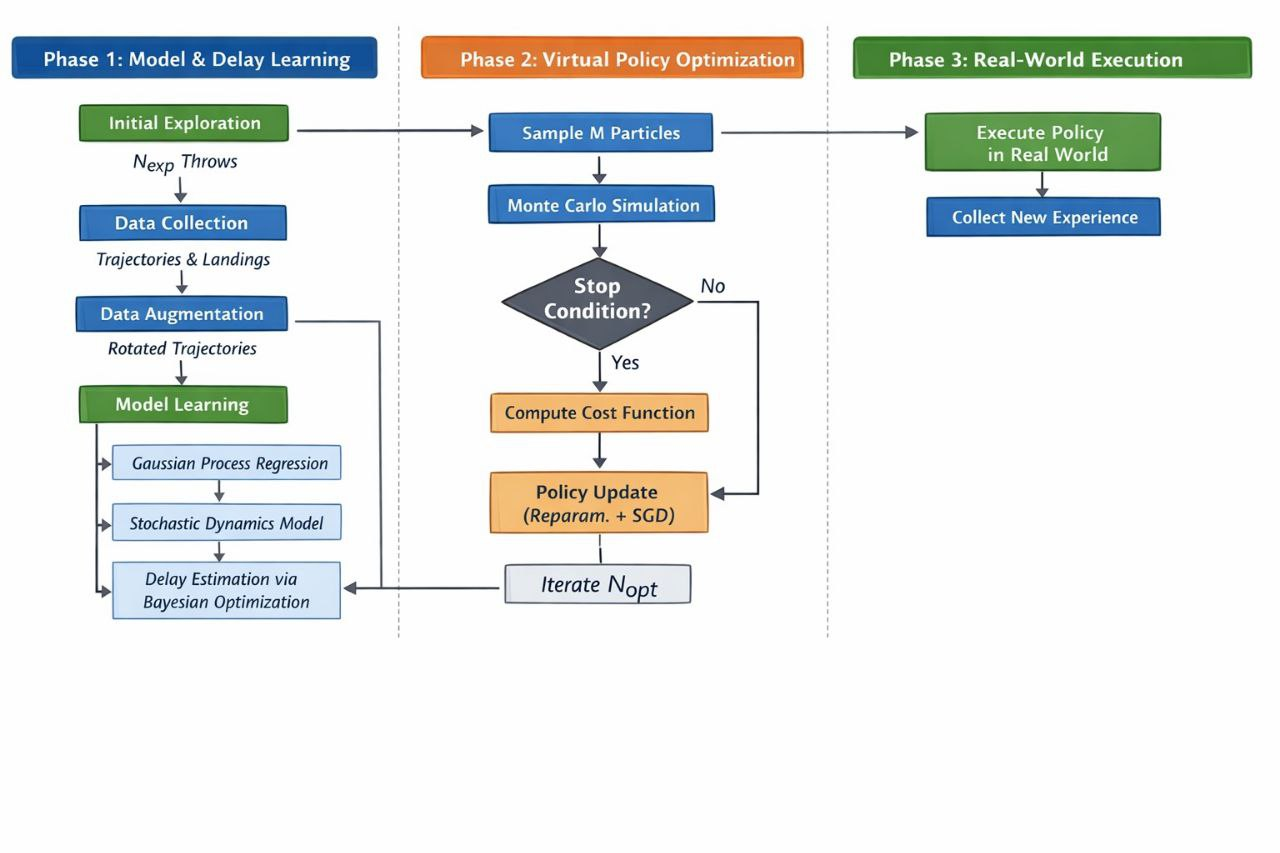
\includegraphics[width=0.90\paperwidth, height=\paperheight, keepaspectratio]{methodology.jpg}
    \end{center}
\end{frame}
\begin{frame}{Baseline: MC-PILOT \textnormal{\small{(Turcato et al., 2025)}}}
    \begin{block}{Core Algorithm}
        \begin{itemize}
            \item \textbf{Model-Based RL} (MBRL): learns a stochastic \textbf{Gaussian Process} model of free-flight object dynamics from $\sim$10 real throws
            \item Policy $\pi_\theta(P) \rightarrow v$: scalar release velocity for a given target $P$, optimised via \textbf{Monte Carlo policy gradient} over GP-simulated particles
            \item Stochastic \textbf{gripper opening delay} $t_d \sim \mathcal{U}(a,a+b)$ estimated via Bayesian Optimisation and propagated through the initial state distribution
            \item Near-\textbf{100\% target accuracy} with $\sim$10 exploration throws vs.\ hundreds for MFRL
        \end{itemize}
    \end{block}
    
\end{frame}
%%%%%%%%%%%%%%%%%%%%%%%%%%%%%%%%%%%%%%%%%%%%%%%%%%%%%%%%%%%%%

\begin{frame}[c]
    \centering
    {\Huge \textbf{Thank You!}}\\[1em]
    {\large Questions \& Discussion}\\[2em]
\end{frame}

%%%%%%%%%%%%%%%%%%%%%%%%%%%%%%%%%%%%%%%%%%%%%%%%%%%%%%%%%%%%%
% \section{Our Proposed Explorations}
% \begin{frame}{Assumptions of MC-PILOT}
%     \begin{alertblock}{Fixed Ground-Level Target Plane}
%         \begin{itemize}
%             \item MC-PILOT fixes all targets on a \textbf{single horizontal ground plane} ($z_P = \text{const}$) with a hard-coded release angle $\alpha \approx 0$ --- designed only for downward-trajectory throws.
%             \item When $z_P$ approaches or exceeds $z_\text{rel} = 1.50$\,m, upward momentum is required --- fixed $q_\text{rel}$ and fixed $\alpha$ make this \textbf{kinematically infeasible} given Panda's stringent joint limits.
%             \item \textbf{Goal:} identify the feasibility boundary as $z_P$ increases and develop a modified framework for targets \textbf{above the robot's release plane}.
%         \end{itemize}
%     \end{alertblock}
%     \begin{alertblock}{No Wind or Environmental Disturbances}
%         \begin{itemize}
%             \item MC-PILOT uses the standard drag equation for \textbf{calm, still air} only --- all experiments are conducted in a controlled indoor lab with no lateral airflow, gusts, or turbulence.
%             \item In semi-outdoor deployments (warehouses, disaster response), even modest wind can shift a lightweight object's landing beyond the success threshold.
%             \item \textbf{Goal:} quantify accuracy degradation under wind and study whether the GP model can \textbf{implicitly absorb} wind effects from data, or whether an explicit wind-state input is required.
%         \end{itemize}
%     \end{alertblock}
% \end{frame}
\section{Our Proposed Explorations}

\begin{frame}{Fixed Ground-Level Target Plane}
    \begin{alertblock}{Assumption}
        \begin{itemize}
            \item MC-PILOT fixes all targets on a \textbf{single horizontal ground plane} ($z_P = \text{const}$) with a hard-coded release angle $\alpha \approx 0$ --- designed only for downward-trajectory throws.
            \item When $z_P$ approaches or exceeds $z_\text{rel} = 1.50$\,m, upward momentum is required --- fixed $q_\text{rel}$ and fixed $\alpha$ make this \textbf{kinematically infeasible} given Panda's stringent joint limits.
        \end{itemize}
    \end{alertblock}
    \begin{block}{Proposed Modification: Elevated Targets}
        \begin{itemize}
            \item \textbf{Expanded policy:} $\pi_\theta(P) \rightarrow [z_P,\ \alpha,\ v]$ --- release height, throw angle, and velocity are \textbf{jointly optimised}, allowing dynamic reconfiguration of $q_\text{rel}$ for each target height.
            \item \textbf{Modified cost:} $\Sigma_c = \text{diag}\!\left(0,\ \tfrac{1}{\ell_c},\ \tfrac{1}{\ell_c}\right)$ minimises lateral ($y$) and vertical ($z$) error, extending to \textbf{arbitrary target planes}.
            \item Redefine $\mathcal{D}_P$ to include $z_P > z_\text{rel}$; study feasibility boundary within Panda joint limits.
        \end{itemize}
    \end{block}
\end{frame}

\begin{frame}{Wind Modelling \& Environmental Disturbances}
    \begin{alertblock}{Problem Context}
        \begin{itemize}
            \item The standard MC-PILOT model assumes \textbf{calm, still air}, limiting reliability in semi-outdoor deployments where modest wind can shift lightweight payloads.
        \end{itemize}
    \end{alertblock}
    \begin{block}{Experimental Setup}
        \begin{itemize}
            \item Extended the physics simulator with a \textbf{wind force term} integrated into the aerodynamic drag equation.
            \item Evaluated against three dynamic wind conditions: \textbf{constant wind}, \textbf{random gusts} (step changes in $\mathbf{w}$), and \textbf{turbulence} (Gaussian noise on $\mathbf{w}$).
            \item Compared a standard \textbf{Wind-Blind} model (8D state) against a \textbf{Wind-Aware} model (10D state with explicit wind input) to determine if the GP implicitly absorbs disturbances.
        \end{itemize}
    \end{block}
\end{frame}

\begin{frame}{Empirical Findings: Wind-Aware vs. Wind-Blind}
    \begin{block}{Key Results}
        \begin{itemize}
            \item \textbf{Accuracy Degradation:} Constant wind degrades base performance (Hit rate dropped from 73\% to 47\% under strong wind).
            \item \textbf{Implicit Absorption:} Surprisingly, the \textbf{Wind-Blind (8D)} model consistently \textbf{outperformed} the Wind-Aware (10D) model across all dynamic conditions.
            \item For example, in Turbulence (W3), the blind baseline achieved a 60\% hit rate compared to the aware model's 47\%.
        \end{itemize}
    \end{block}
    \begin{alertblock}{Conclusion}
        Expanding the state space to 10D increased the learning complexity beyond what the GP could efficiently sample within limited trials. The 8D model was robust enough to implicitly absorb the wind disturbances as a bias term.
    \end{alertblock}
\end{frame}

\begin{frame}{Performance Analysis: Hit Rates}
    \begin{figure}
        \centering
        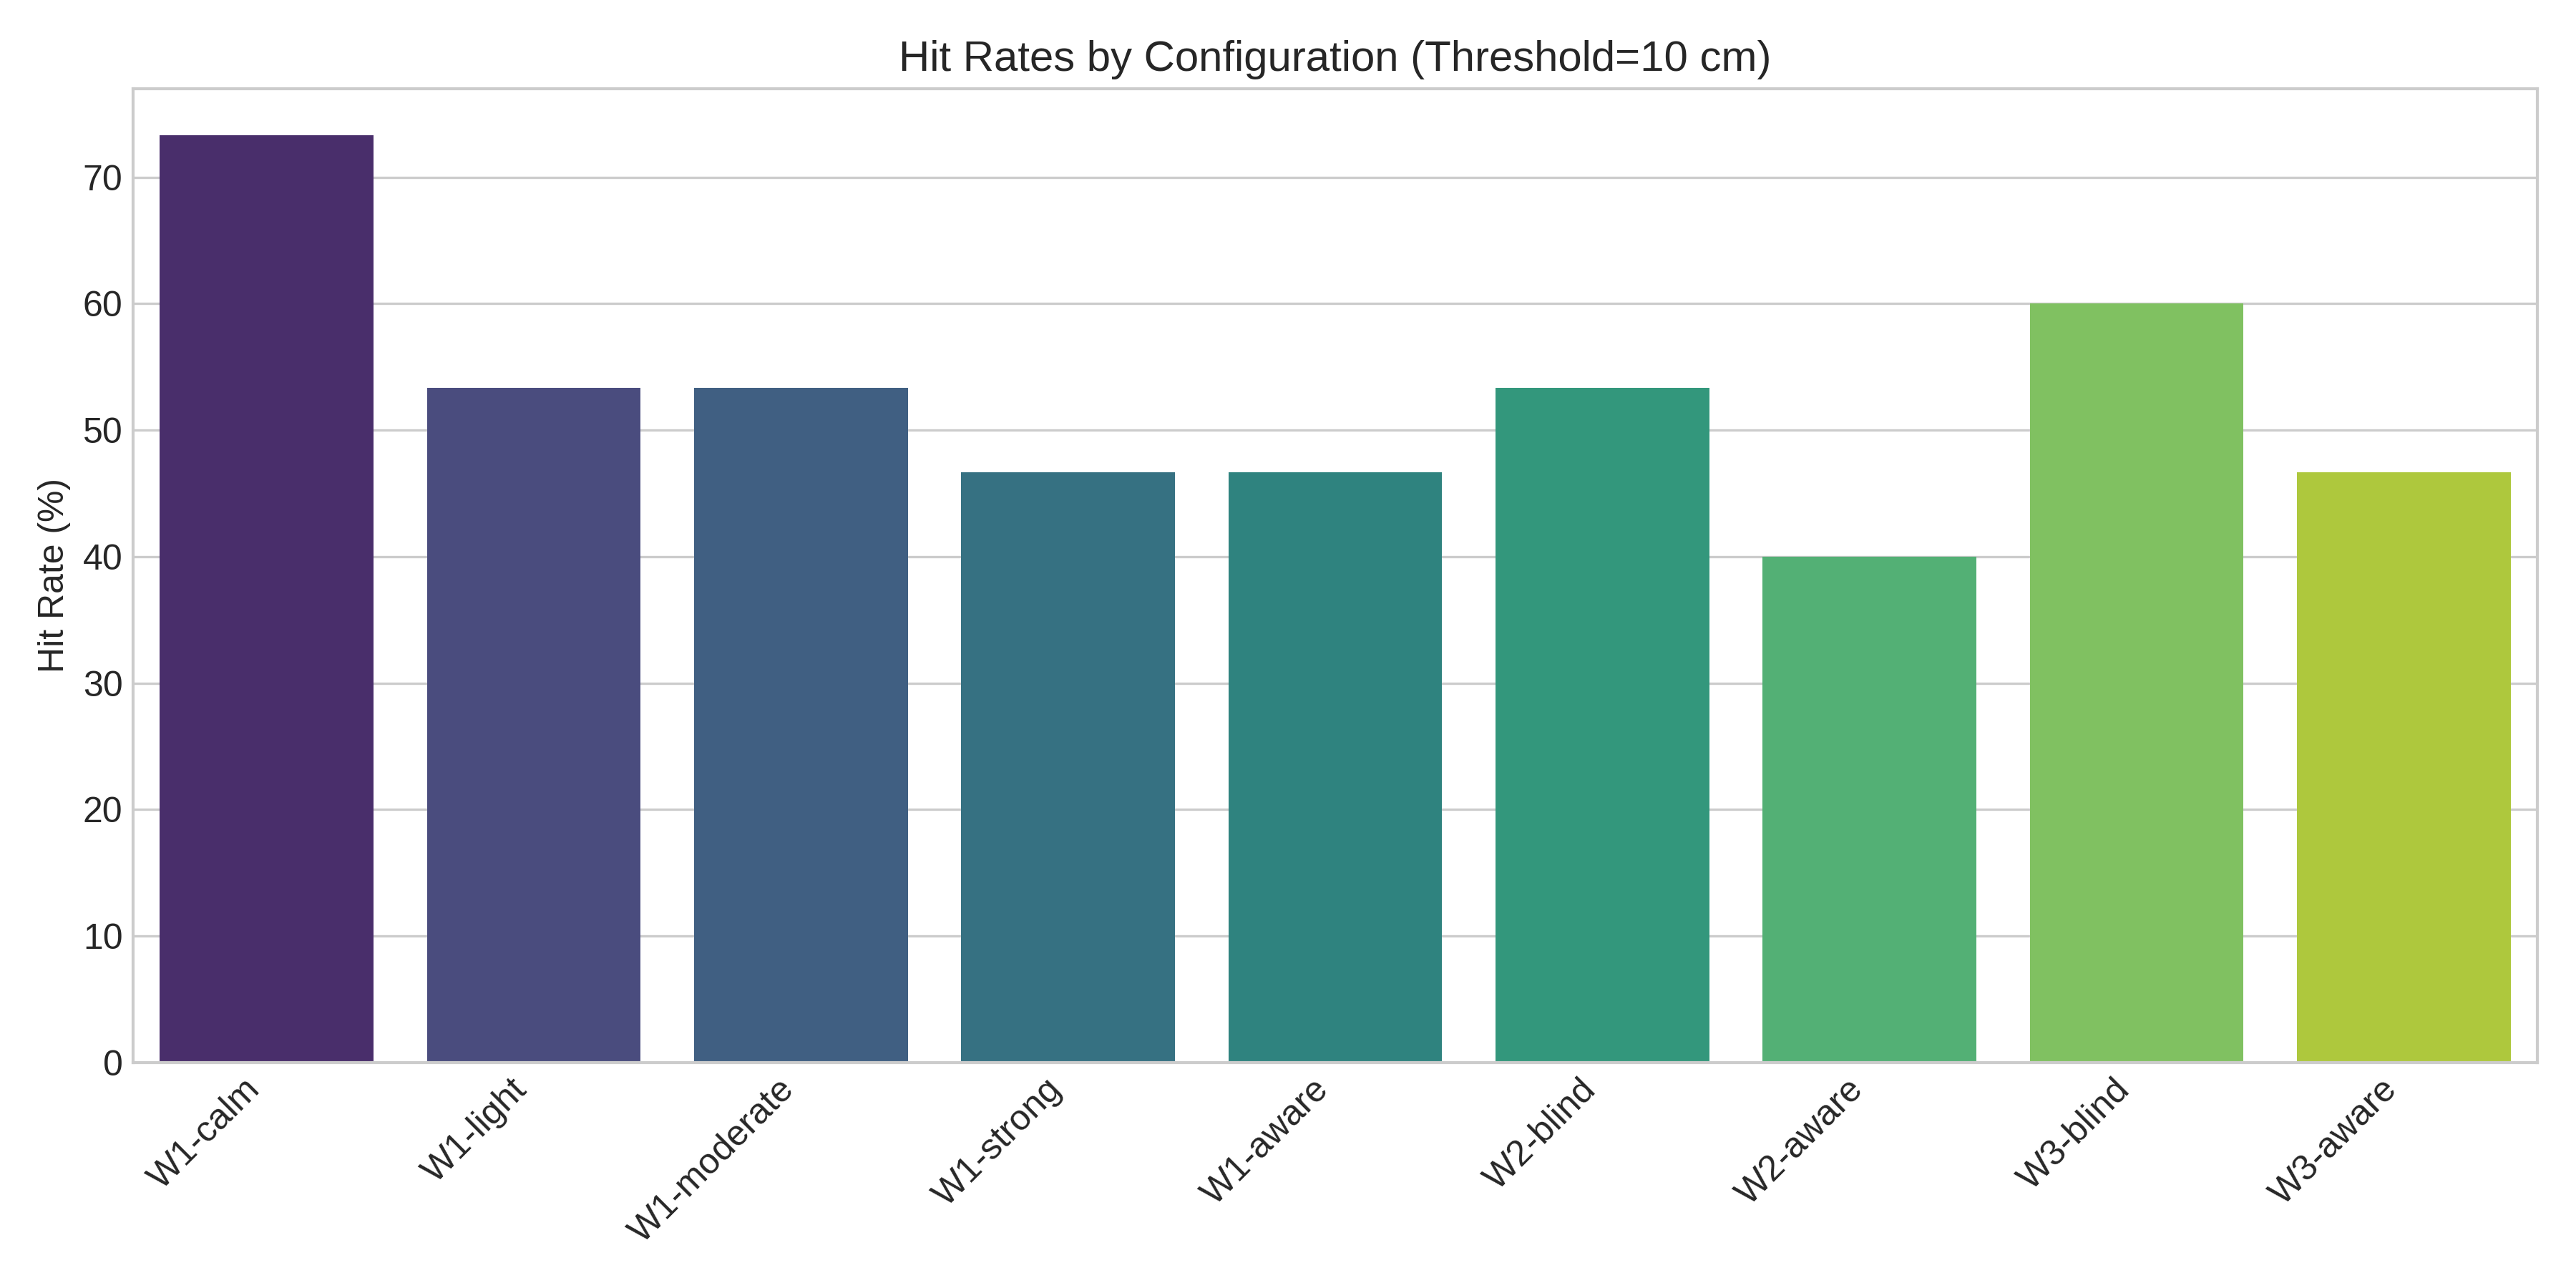
\includegraphics[width=0.85\textwidth]{performance_analysis_plots/hit_rates.png}
        \caption{Comparison of Hit Rates (landing within 10cm threshold) across configurations.}
    \end{figure}
\end{frame}

\begin{frame}{Performance Analysis: Error Variance}
    \begin{figure}
        \centering
        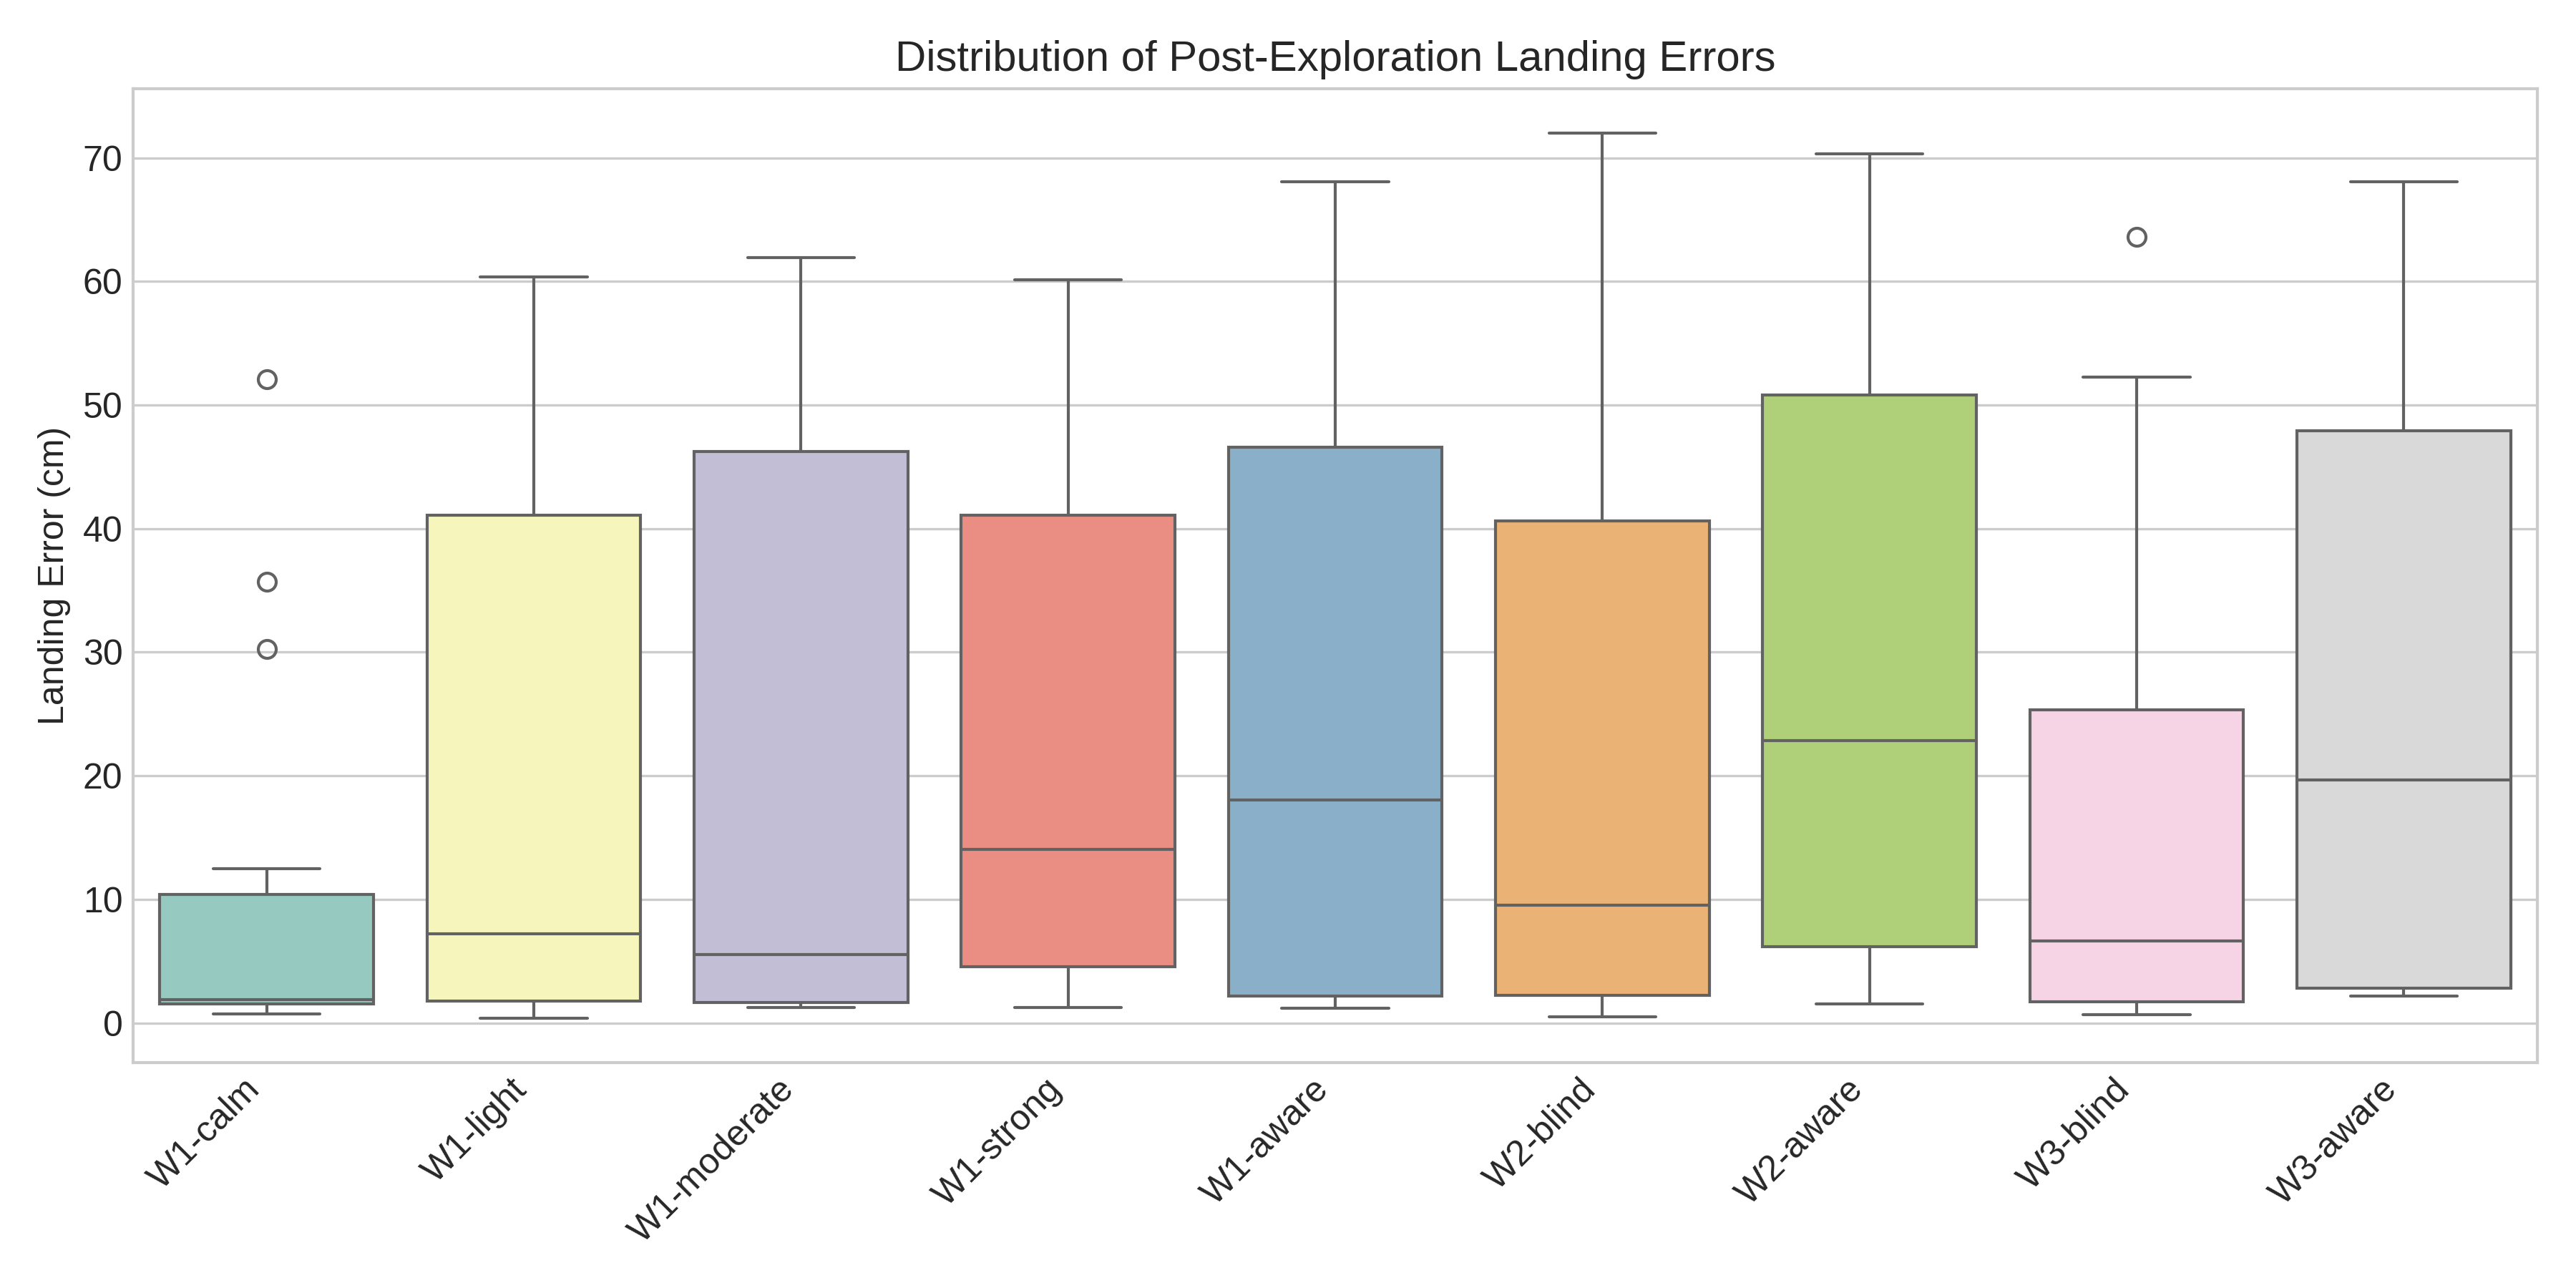
\includegraphics[width=0.85\textwidth]{performance_analysis_plots/error_distributions_boxplot.png}
        \caption{Landing Error Variance and Distribution for post-exploration trials.}
    \end{figure}
\end{frame}

\begin{frame}{Performance Analysis: Learning Convergence}
    \begin{figure}
        \centering
        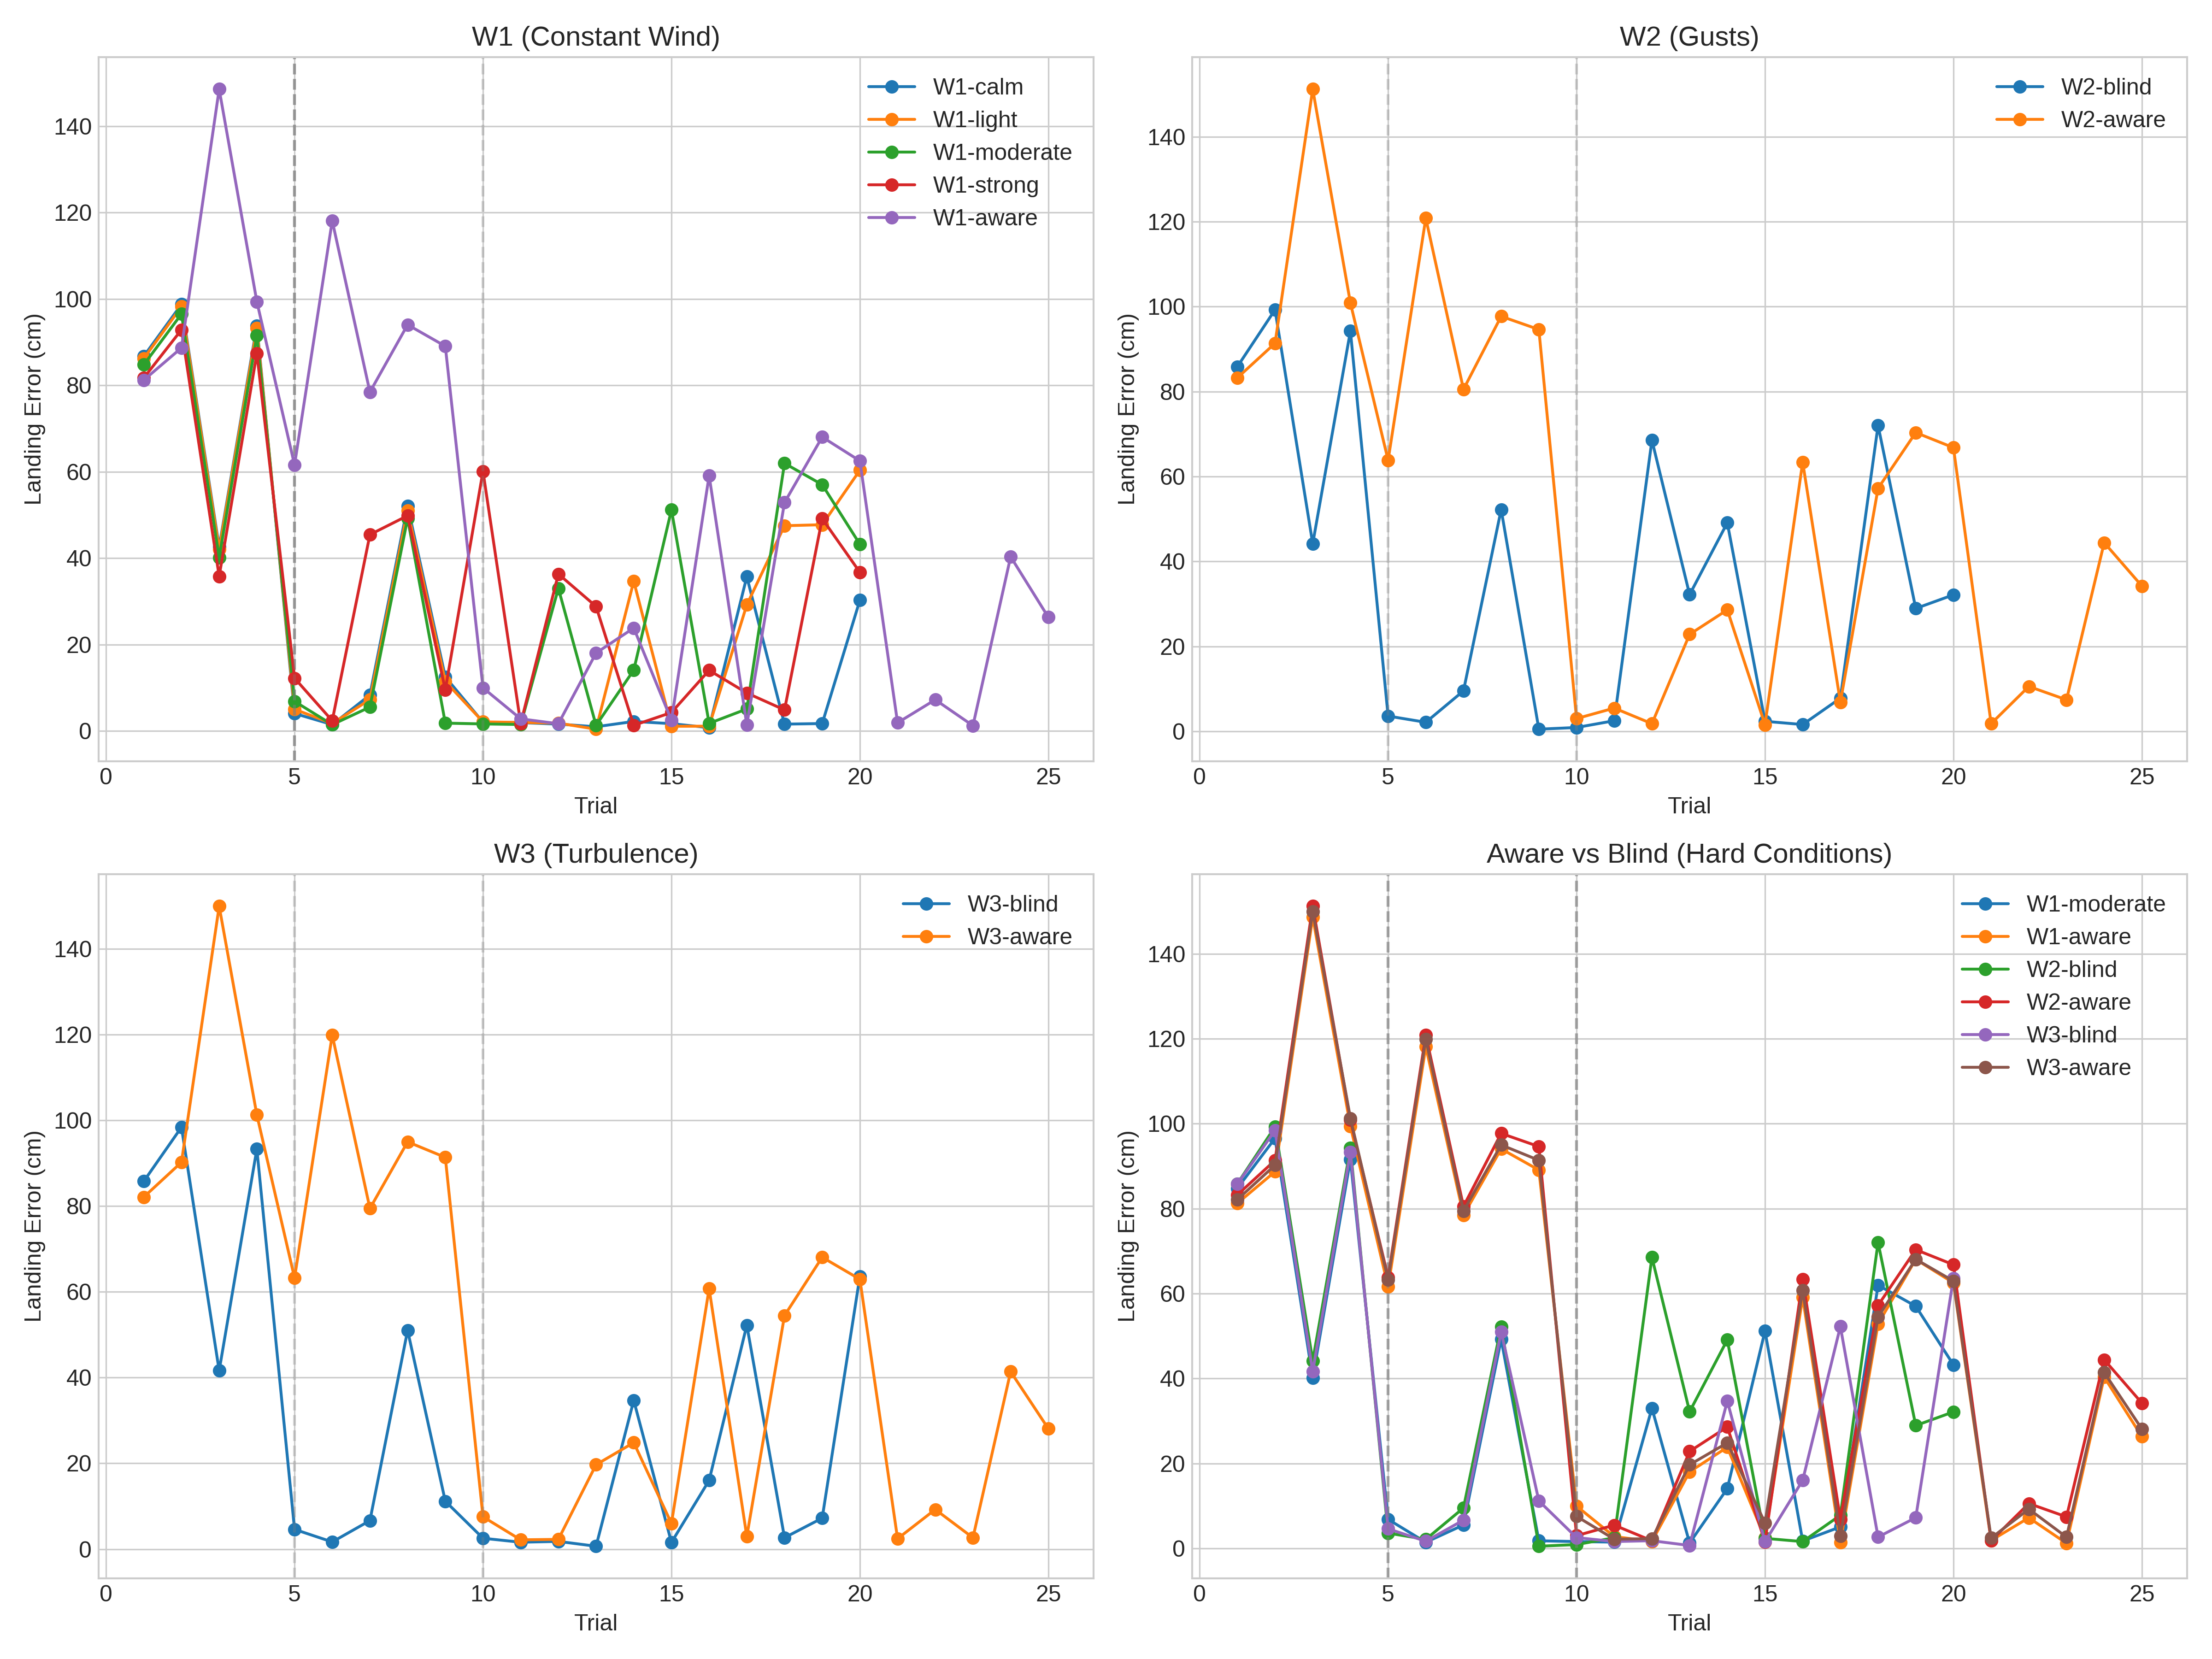
\includegraphics[width=0.85\textwidth]{performance_analysis_plots/learning_curves_error.png}
        \caption{Physical mean error convergence over successive optimization trials.}
    \end{figure}
\end{frame}

\begin{frame}{Performance Analysis: Target Landing Distributions}
    \begin{figure}
        \centering
        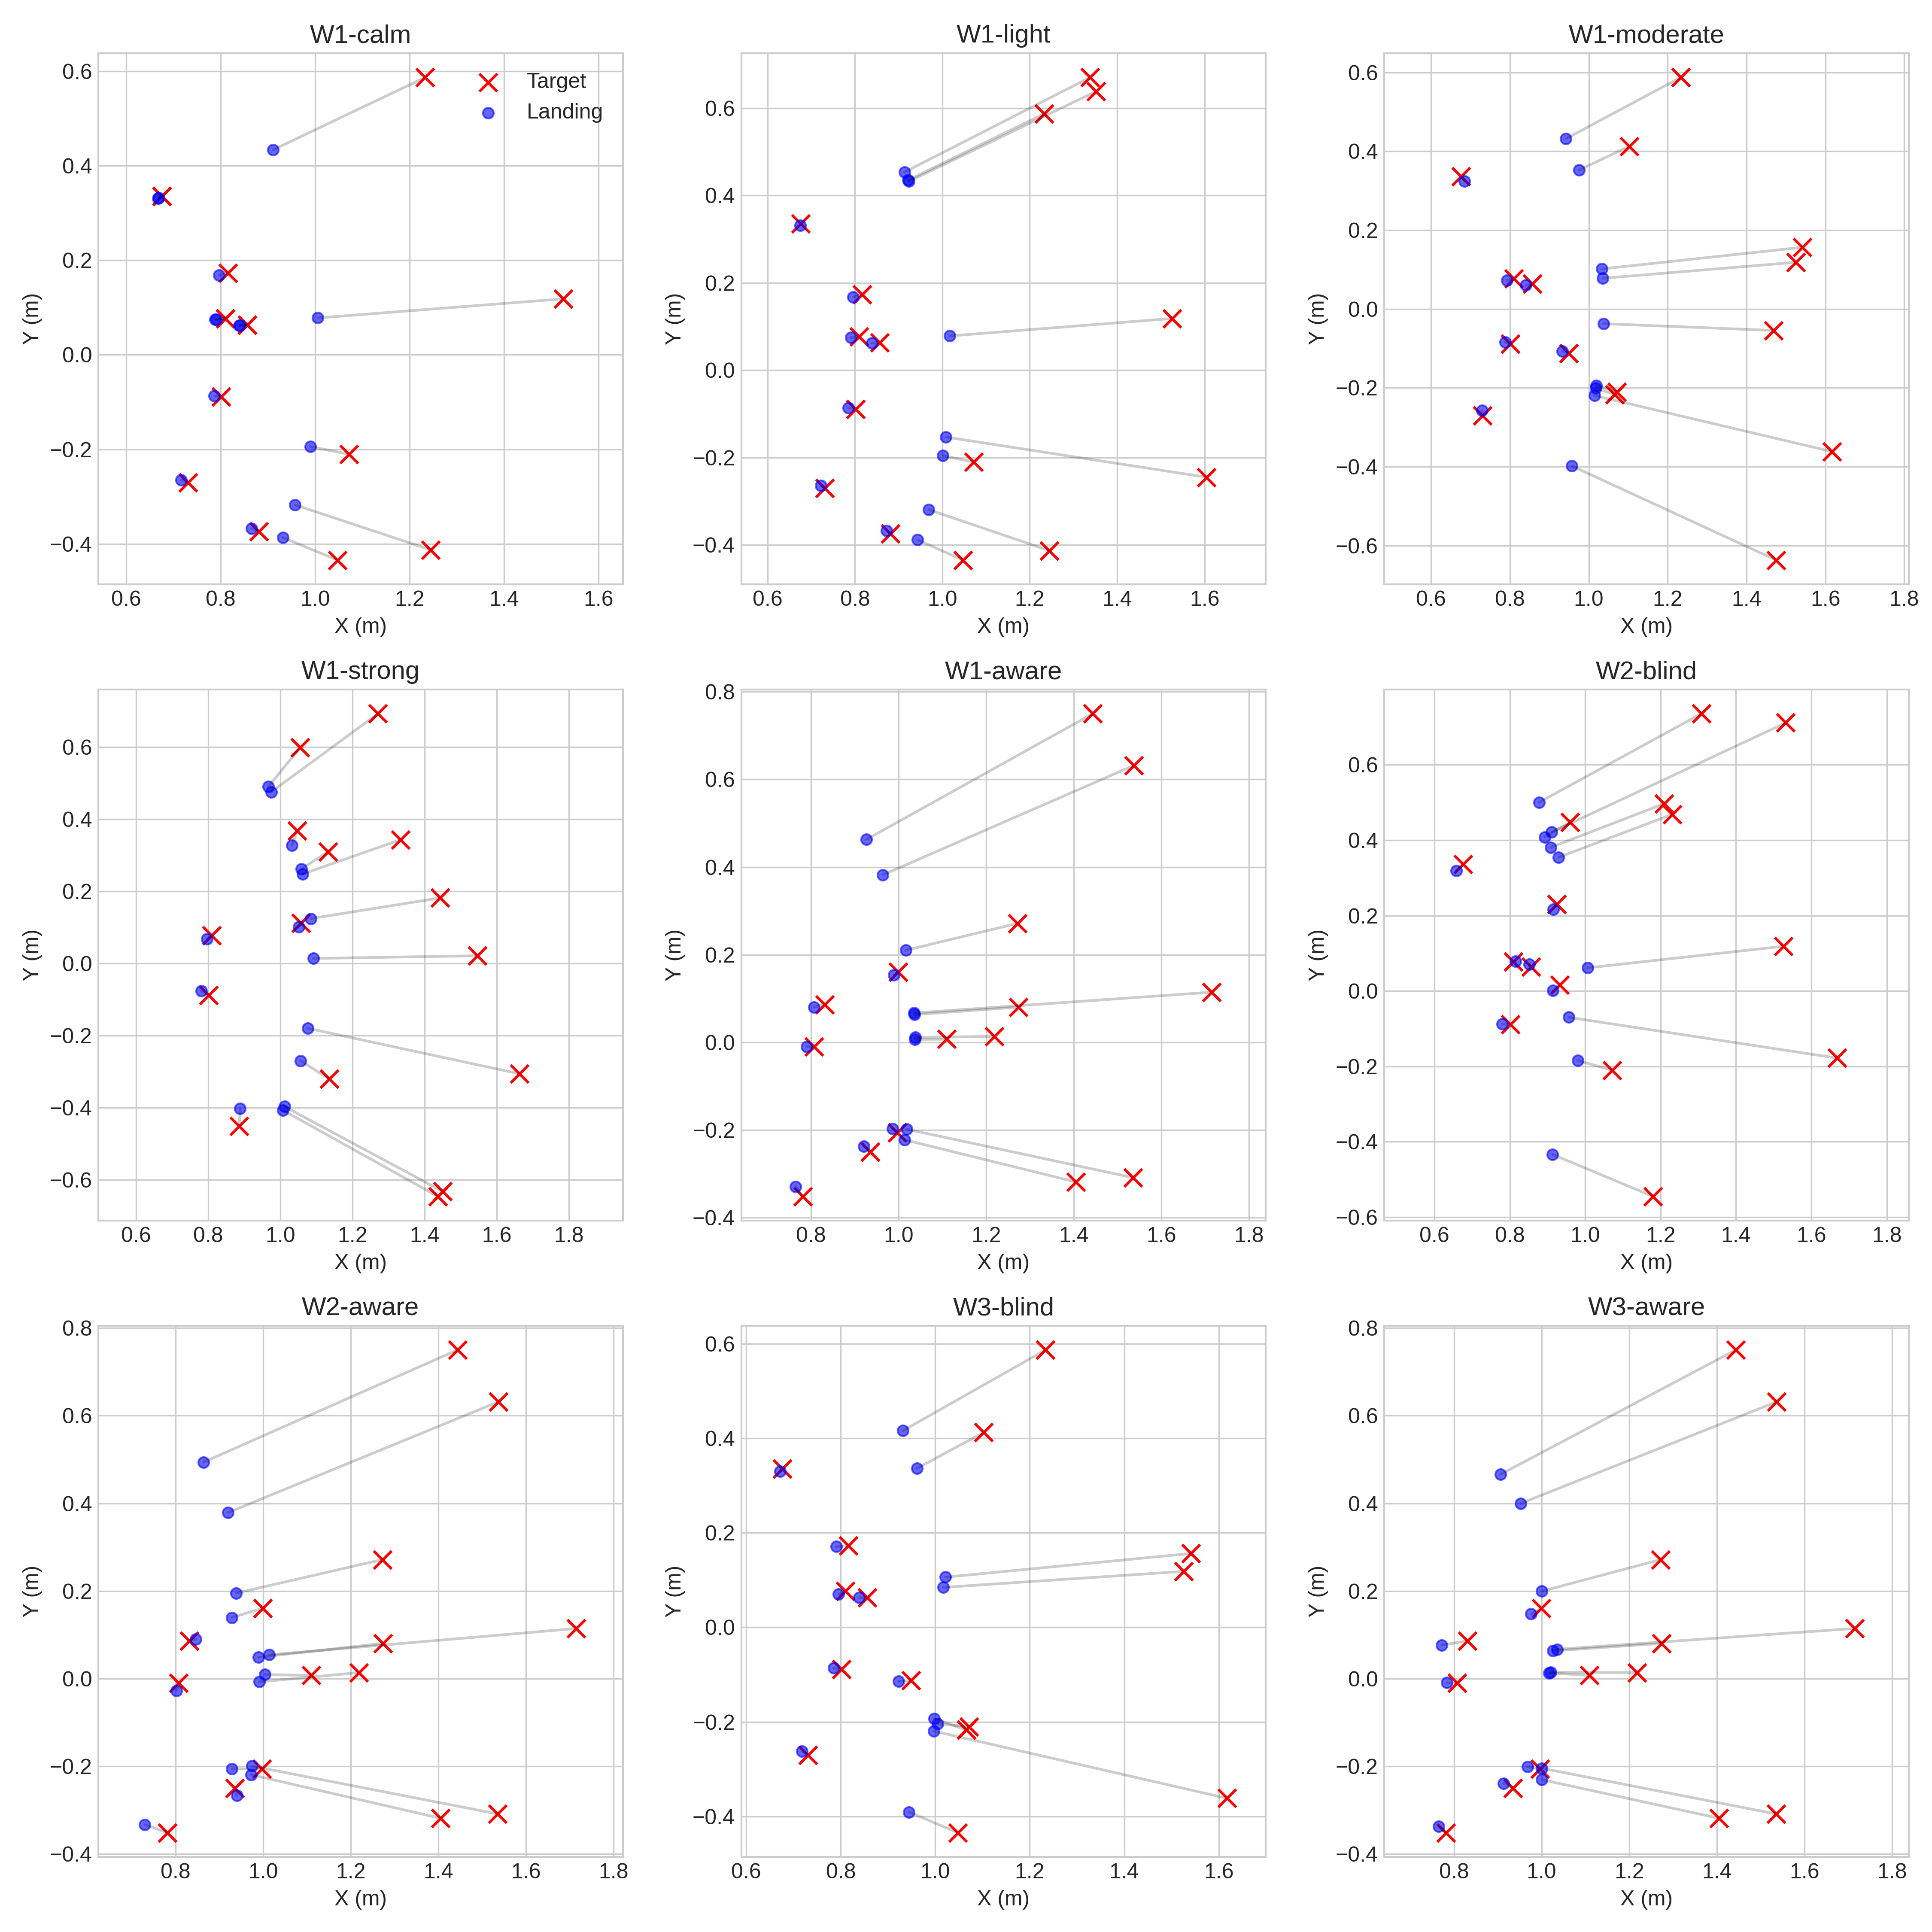
\includegraphics[width=0.85\textwidth]{performance_analysis_plots/scatter_2d_landings.png}
        \caption{2D mapping of actual landing coordinates relative to target positions.}
    \end{figure}
\end{frame}



%%%%%%%%%%%%%%%%%%%%%%%%%%%%%%%%%%%%%%%%%%%%%%%%%%%%%%%%%%%%%
% \begin{frame}{Proposed Modifications: Elevated Targets}
%     \begin{block}{Expanded Action Space}
%         \begin{itemize}
%             \item \textbf{Our policy:} $\pi_\theta(P) \rightarrow [z_P,\ \alpha,\ v]$ \quad --- release height, throw angle, and velocity are all \textbf{jointly optimised}
%             \item This allows the arm to \textbf{dynamically reconfigure} $q_\text{rel}$ for each target height, enabling upward trajectories that the original fixed configuration cannot produce
%         \end{itemize}
%     \end{block}
%     \begin{block}{Modified Cost Function for Vertical Targets}
%         \begin{itemize}
%             \item \textbf{Our cost (vertical/elevated target):} $\Sigma_c = \text{diag}\!\left(0,\ \tfrac{1}{\ell_c},\ \tfrac{1}{\ell_c}\right)$ \quad minimises lateral ($y$) and vertical ($z$) error at a fixed horizontal distance
%             \item Seamlessly extends to \textbf{arbitrary target planes} by choosing the appropriate diagonal entries
%         \end{itemize}
%     \end{block}
%     \begin{block}{Modification 3 --- Target Domain Expansion}
%         Redefine $\mathcal{D}_P$ to include $z_P > z_\text{rel}$; study feasibility boundary and require new $q_\text{rel}$ configurations within Panda joint limits.
%     \end{block}
% \end{frame}

% \begin{frame}{Proposed Modifications: Wind Modelling}
%     \begin{block}{Wind Force in Simulation}
%         \begin{itemize}
%             \item Extend Gazebo physics with a \textbf{wind force term} added to the drag equation.
%             \item Three wind scenarios: \textbf{constant wind}, \textbf{random gusts} (step changes in $\mathbf{w}$), \textbf{turbulence} (Gaussian noise on $\mathbf{w}$)
%         \end{itemize}
%     \end{block}
%     % \begin{block}{Research Questions}
%     %     \begin{columns}[T]
%     %         \begin{column}{0.48\textwidth}
%     %             \textbf{Q1: Can MC-PILOT's GP absorb wind implicitly?}
%     %             \begin{itemize}
%     %                 \item Retrain GP on trajectories collected under wind
%     %                 \item Test whether the learned dynamics implicitly correct for a consistent wind direction without explicit wind state
%     %             \end{itemize}
%     %         \end{column}
%     %         \begin{column}{0.48\textwidth}
%     %             \textbf{Q2: Is explicit wind state needed?}
%     %             \begin{itemize}
%     %                 \item Extend augmented state $\tilde{x}_{t'}$ with measured or estimated wind vector $\mathbf{w}$
%     %                 \item Compare accuracy with and without wind state as GP input; benchmark against PPO/SAC
%     %             \end{itemize}
%     %         \end{column}
%     %     \end{columns}
%     % \end{block}
% \end{frame}

%%%%%%%%%%%%%%%%%%%%%%%%%%%%%%%%%%%%%%%%%%%%%%%%%%%%%%%%%%%%%
\section{Literature Survey}

\begin{frame}{Literature Survey}
        \textbf{Primary Baseline (MBRL for PnT)}
        \begin{itemize}
            \item \textbf{Turcato et al.\ (2025)} --- \textit{MC-PILOT}: GPR dynamics + Monte Carlo policy gradient + Bayesian delay estimation; near-100\% accuracy with $\sim$10 throws
            \item Amadio et al.\ (2022) --- \textit{MC-PILCO}: parent MBRL algorithm; model-based policy search with Monte Carlo gradient estimation
        \end{itemize}
        \vspace{0.3em}
        \textbf{Model-Free PnT}
        \begin{itemize}
            \item Zeng et al.\ (2020) --- \textit{TossingBot}: end-to-end deep RL; effective but requires hundreds of trials
            % \item Fang et al.\ (2021) --- DQN + DDPG; fixed target grid
            % \item Bianchi et al.\ (2023) --- PPO with soft robot; fixed targets
        \end{itemize}
        \textbf{Extended PnT: Cluttered Scenes \& Landing Pose}
    \begin{itemize}
        \item Kasaei \& Kasaei\ (ICRA 2024) --- \textit{Push-Grasp-Throw}: model-free deep RL that combines non-prehensile pushing with grasping and throwing to handle cluttered scenarios; extends the robot's operational reach while isolating target objects via push reconfiguration
        \item Liu et al.\ (2025) --- \textit{Learning to Throw-Flip}: first work to control landing \textbf{pose} (position \emph{and} orientation), not just position; decouples parasitic rotation via the impulse-momentum principle and combines a physics-based free-flight model with regression-based learning for unmodelled effects
    \end{itemize}
\end{frame}

%%%%%%%%%%%%%%%%%%%%%%%%%%%%%%%%%%%%%%%%%%%%%%%%%%%%%%%%%%%%%
\section{Evaluation Plan}

\begin{frame}{Evaluation Plan and Expected Results}
    \begin{block}{Quantitative Metrics}
        \begin{itemize}
            \item \textbf{Landing Error (m):} mean Euclidean distance between landing point and target.
            \item \textbf{Target Reach Accuracy (\%):} fraction of throws within 0.1\,m of target.
            \item \textbf{Sample Efficiency:} throws required to reach 80\% accuracy --- key MBRL vs.\ MFRL axis.
            \item \textbf{Elevated Target Feasibility:} accuracy vs.\ target height $z_P$; identify kinematic boundary where performance degrades.
            \item \textbf{Wind Robustness:} accuracy vs.\ wind speed $\|\mathbf{w}\|$ for constant / gust / turbulence; MC-PILOT vs.\ PPO/SAC degradation curves.
        \end{itemize}
    \end{block}
    \begin{block}{Expected Visualisations}
        \begin{itemize}
            \item \textbf{Accuracy vs.\ training throws}: PPO, SAC, MC-PILOT, MC-PILOT + our modifications
            \item \textbf{2D landing scatter plots}: ground vs.\ elevated targets; calm vs.\ windy conditions
            \item \textbf{Accuracy vs.\ wind speed:} degradation onset and relative MBRL/MFRL robustness
            \item \textbf{Accuracy vs.\ target height $z_P$:} feasibility boundary curve
        \end{itemize}
    \end{block}
\end{frame}
\end{document}